\documentclass{article}
\usepackage[utf8]{inputenc}
\usepackage{graphicx}
\graphicspath{ {images/} }

\title{Análisis de las gráficas de la tarea 3}
\date{}

\begin{document}

\maketitle

Comencemos el análisis de las gráficas obtenidas en la tarea 3. Para el oscilador armónico simple tenemos las gráficas de posición vs tiempo y el diagrama de fase (velocidad vs posición) al igual que para el oscilador amortiguado, todo se realizó para 5 conjuntos de datos diferentes, el único parámetro que mantuve constante fue el tiempo, porque me pareció adecuado para poder analizar los cambios de las gráficas basándome en un parámetro invariante. 

\section{Oscilador amortiguado (posición vs tiempo):}

\begin{figure}[htp]
    \centering
    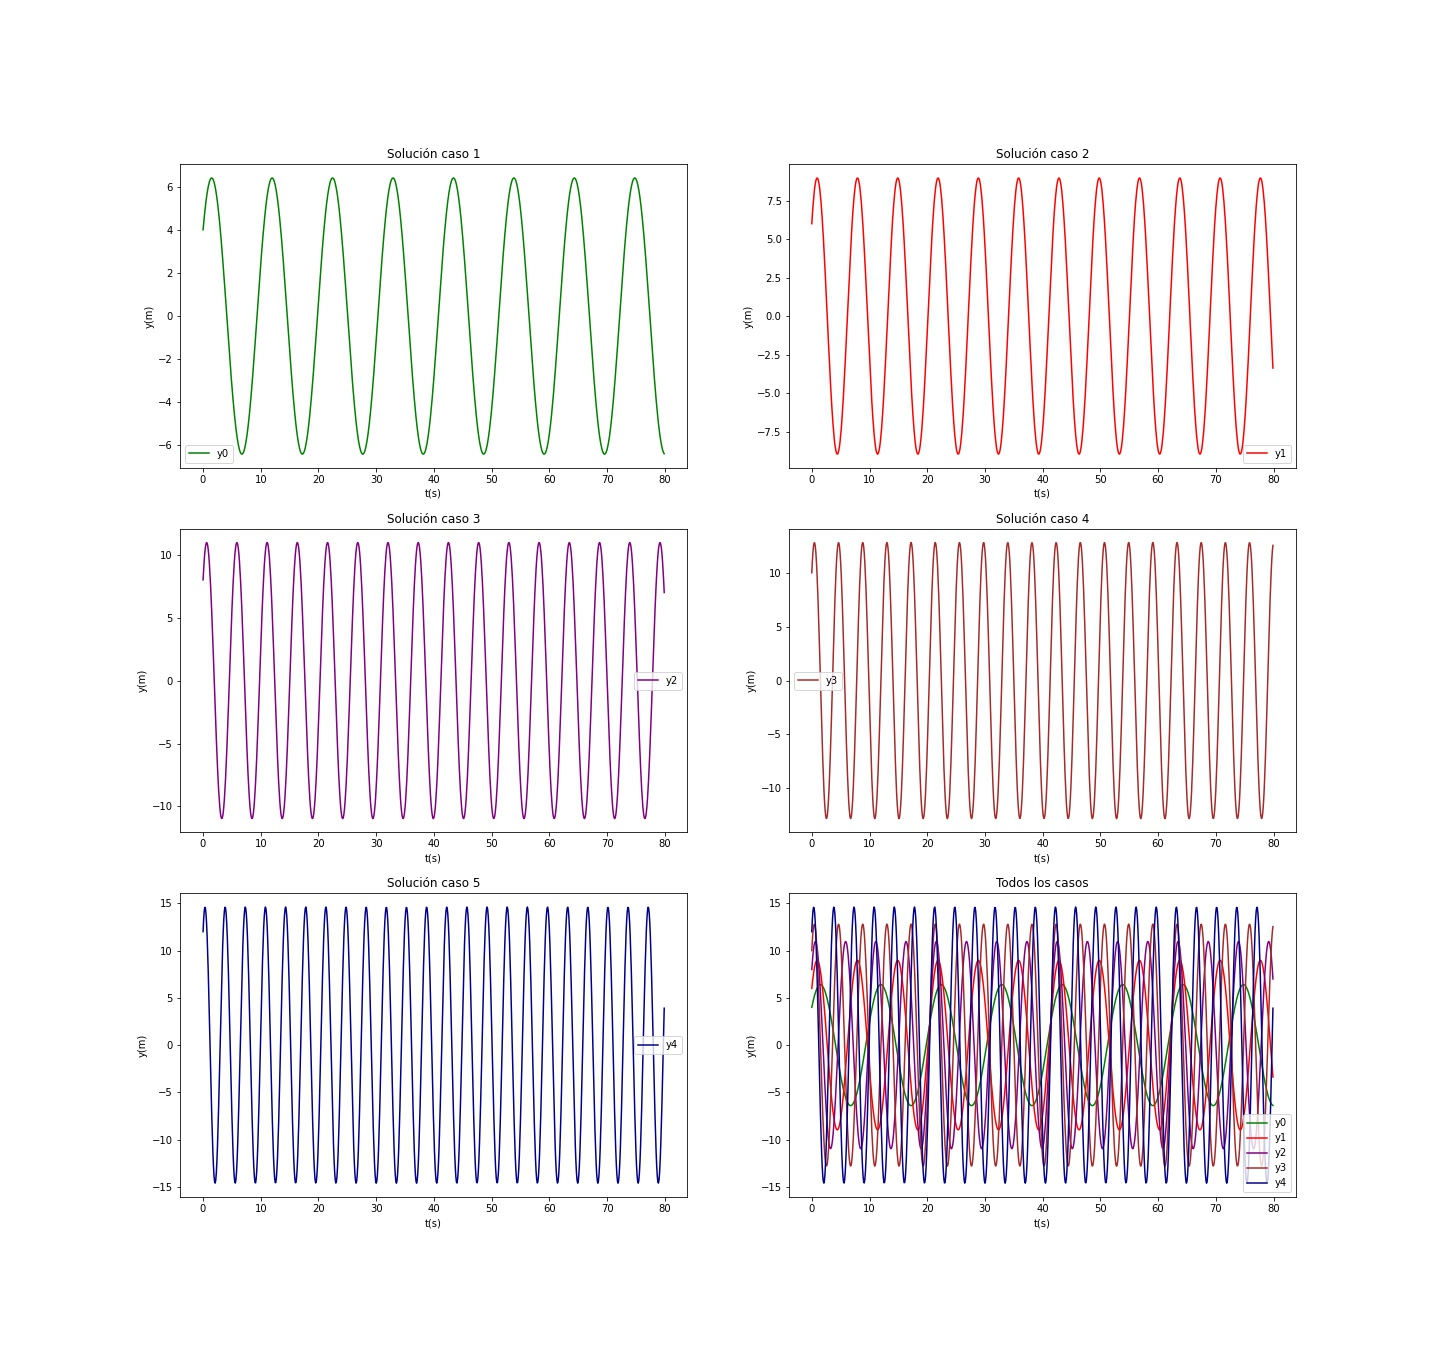
\includegraphics[width=17cm]{Oscilador.jpg}
    \caption{Osciladores armónicos}
    \label{fig:oscilador1}
\end{figure}

En estas gráficas, podemos corroborar las características del oscilador armónico para un sistema masa-resorte, tales como la amplitud constante en todo instante de tiempo $t$ considerado, es decir, la masa se desplaza un $x$ vuelve a su posición de equilibrio para luego contraerse un $-x$.Además, se muestra que existe un período, este período depende exclusivamente de la frecuencia inicial y que el movimiento del sistema se mantendrá siempre y cuando una fuerza externa no actúe sobre él. Se ve claramente que el comportamiento del sistema estará determinado por las condiciones iniciales que se le den, y podrá ser descrito por un coseno o un seno. Se sabe que la solución está dada por $y(t)= A\cos(wt)+B\sin(wt)$ o también lo podemos ver como $y(t)=A\cos(wt+\phi)$ y en las gráficas obtenidas se puede ver claramente este comportamiento.

\subsection{Diagrama de fase oscilador armónico:}
\begin{figure}[htp]
    \centering
    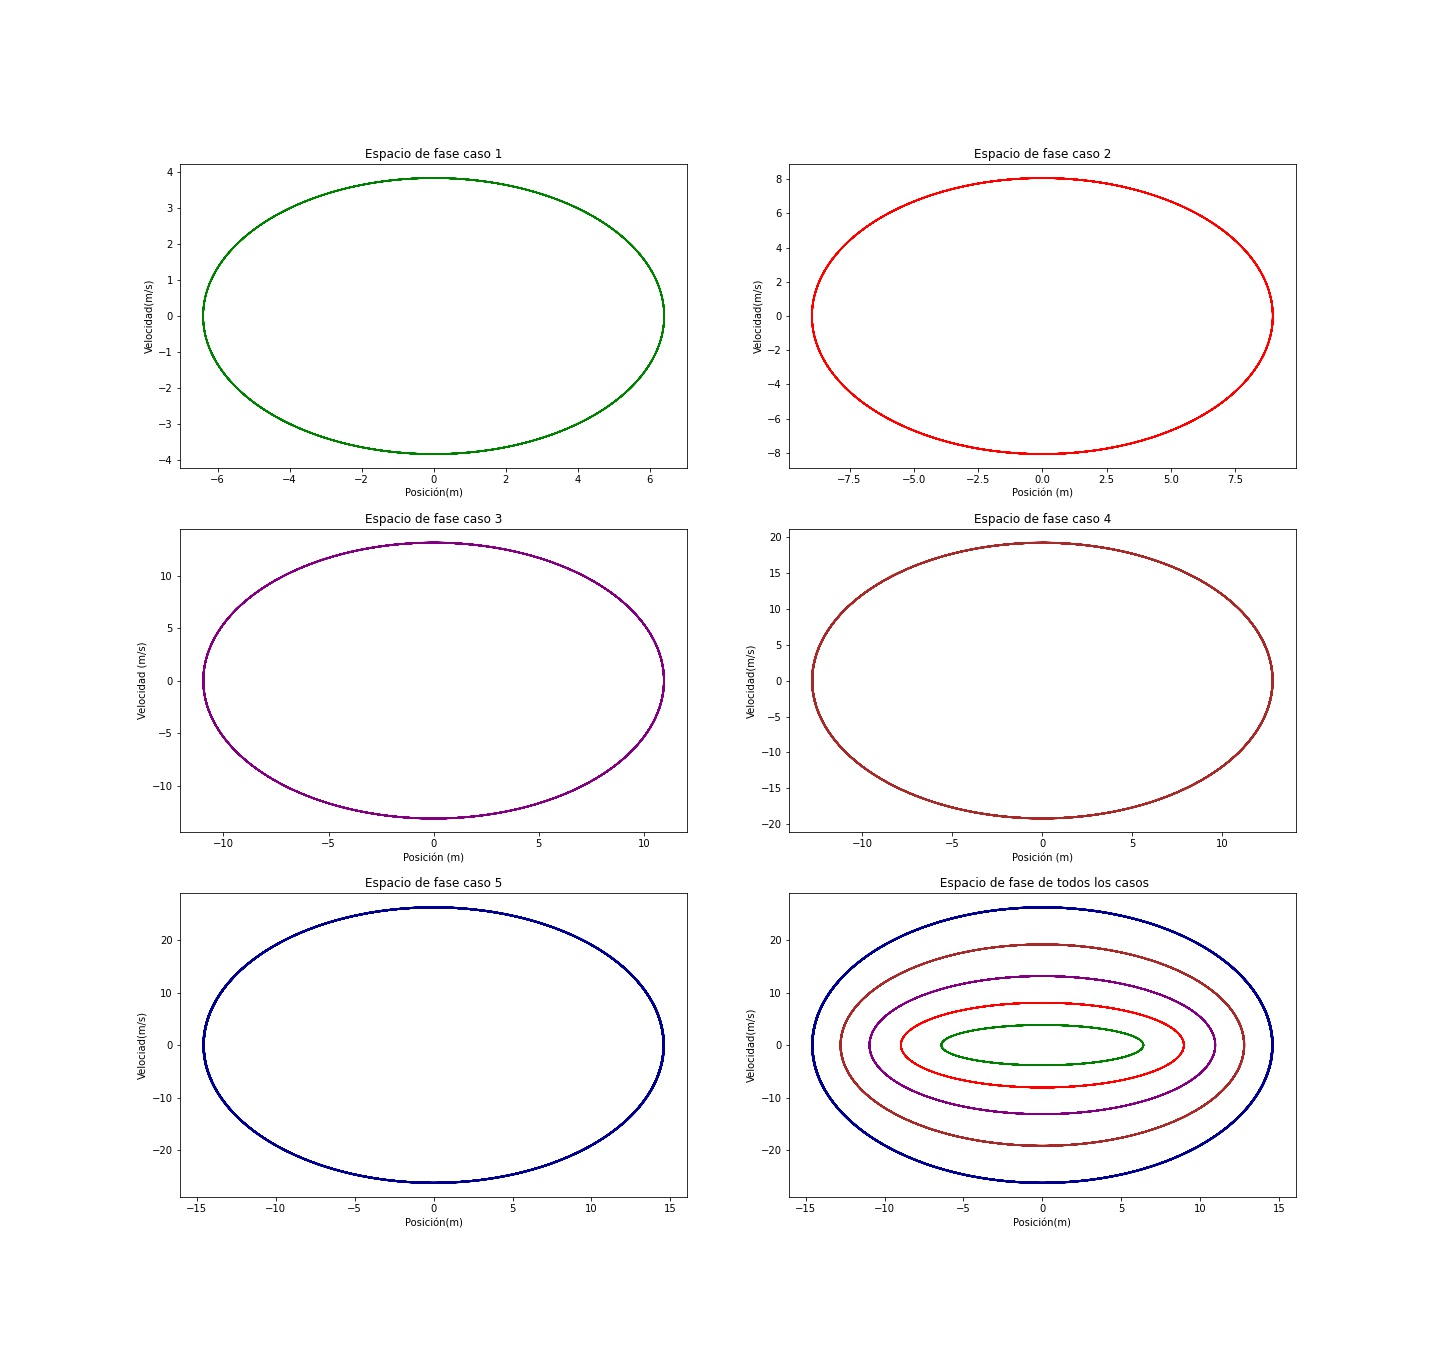
\includegraphics[width=17cm]{Diagfaseoscilador.jpg}
    \caption{Diagramas de fase osciladores armónicos}
    \label{fig:fase1}
\end{figure}

Considerando que para solucionar la ecuación diferencial del sistema masa resorte hicimos una reducción de orden y definimos $\vec{y}=(y,y')$ el plano que difinen $(y,y')$  se conoce como espacio de fase. Conforme $t$ varía estos se mueven a lo largo de un camino de fase dado. Al variar las condiciones iniciales del sistema, el camino cambiará, el total de posibles caminos representa el diagrama de fase, por lo que según las gráficas obtenidas para nuestro sistema podríamos decir que solamente hay un posible camino para las condiciones inciales dadas. \\

Sabiendo que $y(t)= A\cos(wt+\phi)$ y $y'(t)=-Aw\sin(wt+\phi)$ podemos eliminar $t$ y obtener la ecuación de trayectoria: \\ $$\frac{x^2}{A^2}+\frac{x'^2}{w^2A^2}=1$$ 

la cual representa una elipse, reescribiendo en términos de la energía del sistema obtenemos: \\ $$\frac{x^2}{2E/k}+\frac{x'^2}{2E/m}=1 $$ de esta manera la trayectoria representa la energía total del oscilador armónico. Y podemos concluir que al ser representada por una sola trayectoria, la energía total del sistema es constante en cada punto del mismo.

\section{Oscilador amortiguado:}
Para el caso del oscilador amortiguado, sabemos que ahora una fuerza externa, influye sobre el sistema oponiéndose al movimiento y ocasionando que este se detenga. Podemos considerar entonces que para el este sistema masa-resorte esta fuerza es dada por un amortiguador (que puede ser el aire), en las gráficas que encontraremos en la parte inferior evidenciamos como esta fricción ocasiona que a medida que el tiempo avanza, el oscilador comienza a frenarse, su amplitud disminuye hasta ser cero. En este caso, el oscilador sigue teniendo un comportamiento periódico que depende de la frecuencia. \\

Debemos tener en cuenta que las gráficas que obtuvimos son para un oscilador subamortiguado, es decir $\gamma ^2<w^2$. Por lo que la solución general está dada por $y(t)=Ae^{-\gamma t}\cos(wt+\phi)$ y $w=\sqrt{w_{0}^2-\gamma^2}$ donde $w_{0}$ es la frecuencia del oscilador armónico simple. Los otros casos del oscilador amortiguado están dados por: $w_{0}=\gamma^2$ que es el caso crítico y $w_{0}^2<\gamma^2$ el caso sobreamortiguado.

\begin{figure}[htp]
    \centering
    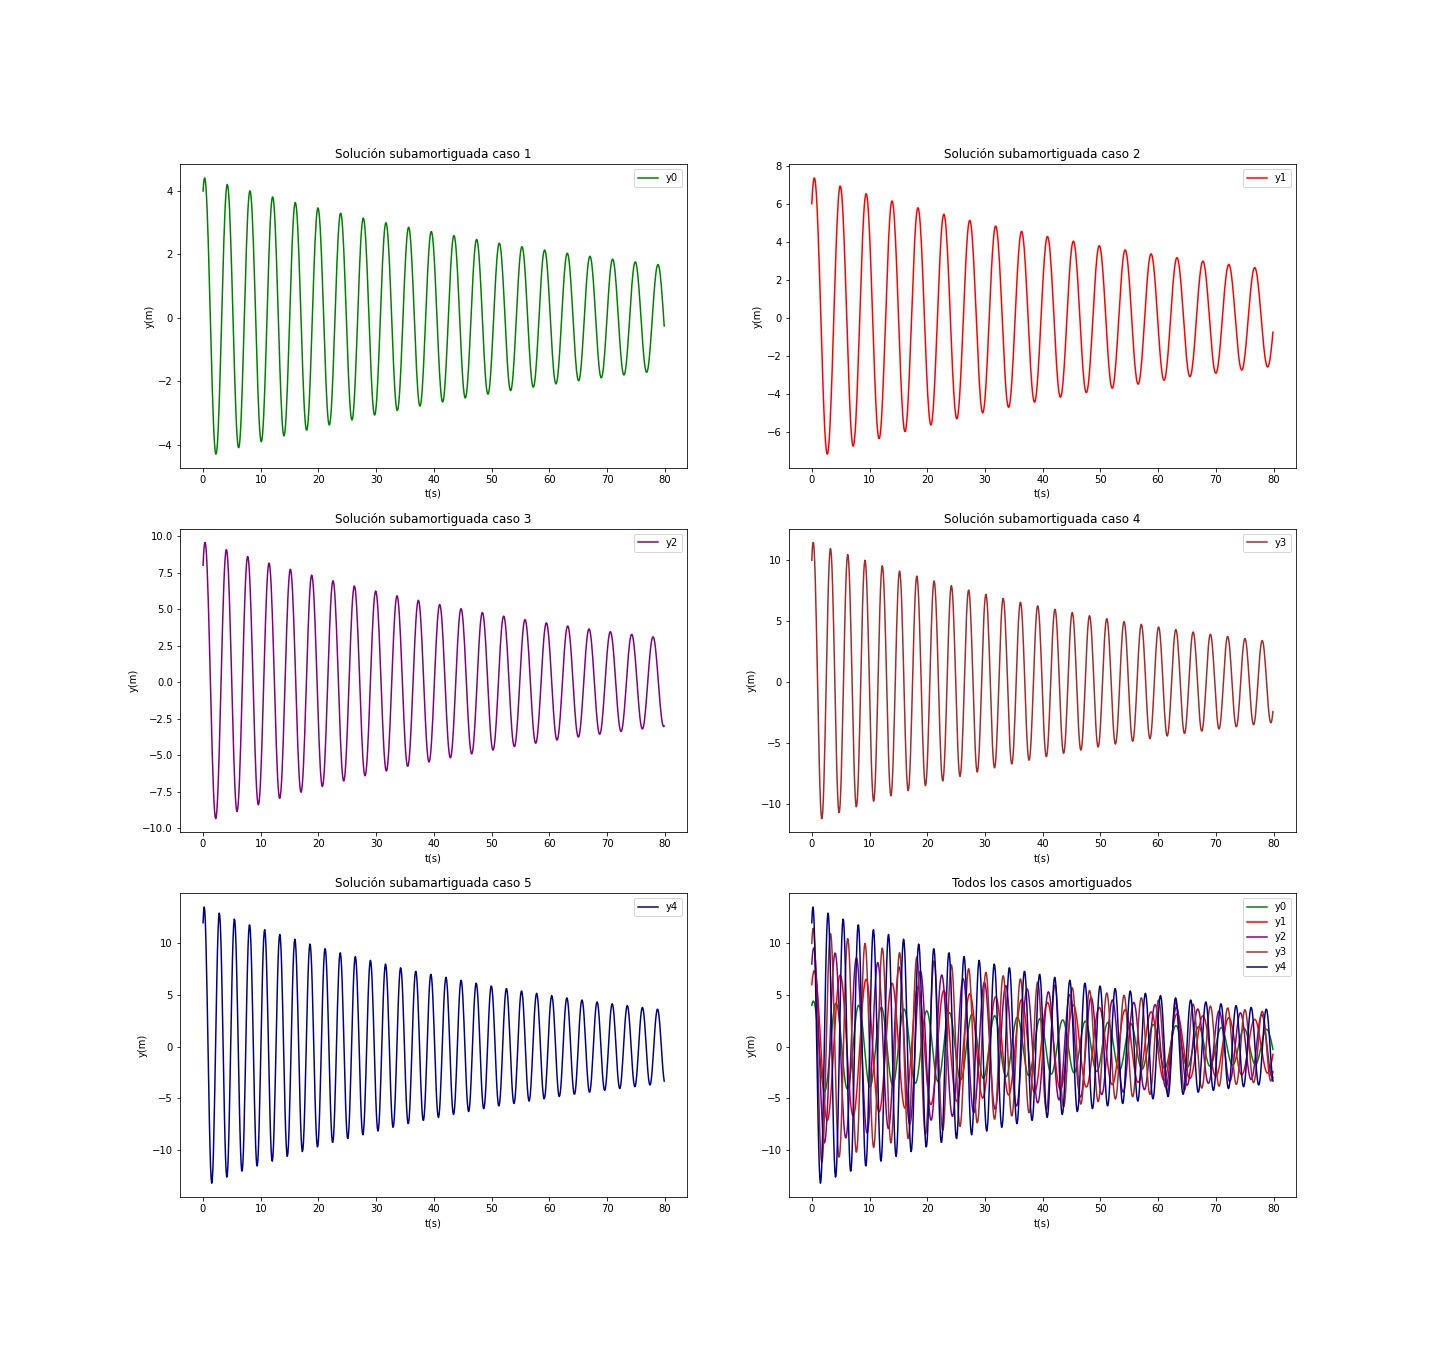
\includegraphics[width=17cm]{Osciladoramortiguado.jpg}
    \caption{Oscilador amortiguado}
    \label{fig:oscilador2}
\end{figure}
\\ \\
\subsection{Diagramas de fase osciladores subamortiguados:}
\begin{figure}[htp]
    \centering
    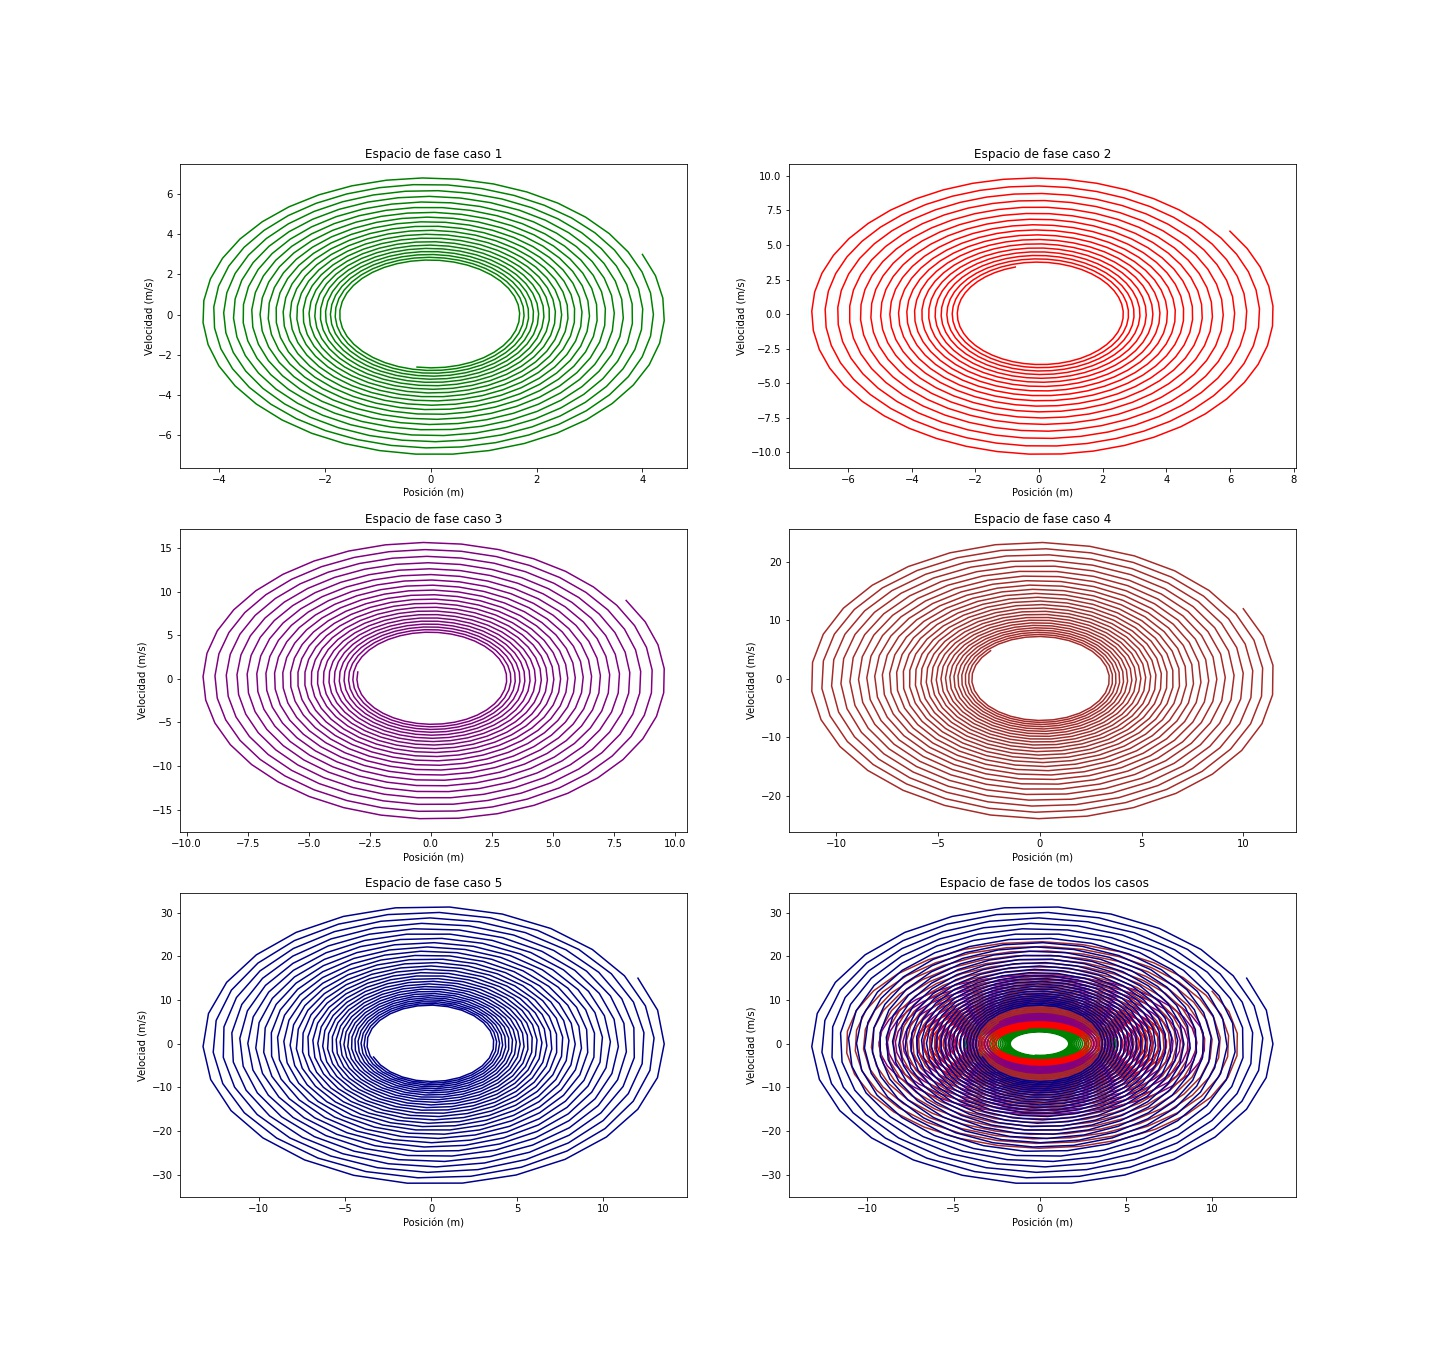
\includegraphics[width=17cm]{Diagfaseosciladoramortiguado.jpg}
    \caption{Oscilador amortiguado}
    \label{fig:fase2}
\end{figure}

Sosteniendo el mismo principio del caso armónico, obtenemos que la ecuación de trayectoria en polares, estará dada por: $\rho=wAe^{-\gamma t}$ la cual representa una espiral logarítmica, esta nos muestra como cada nueva trayectoria la energía del sistema es menor que la anterior.


\end{document}
